% !TEX root = template.tex

\newcommand\mygather{\texttt{MY\_Gather}\xspace}
\newcommand\myscatter{\texttt{MY\_Scatter}\xspace}

\newcommand\mpigather{\texttt{MPI\_Gather}\xspace}
\newcommand\mpiscatter{\texttt{MPI\_Scatter}\xspace}

%----------------------------------------------------------------------
\section{Algorithm \mygather}

%-------
\subsection{Strategy Comparison}

Two different Gather algorithms, one based on Binomial-Trees and one based on a Divide-And-Conquer approach were implemented and tested. Figure \ref{fig:gather:binom_vs_dac} shows the absolute performance of each of the implementations in comparison with the OpenMPI Gather implementation.

\begin{figure}[h]
  \centering
  \begin{subfigure}[b]{0.49\textwidth}
        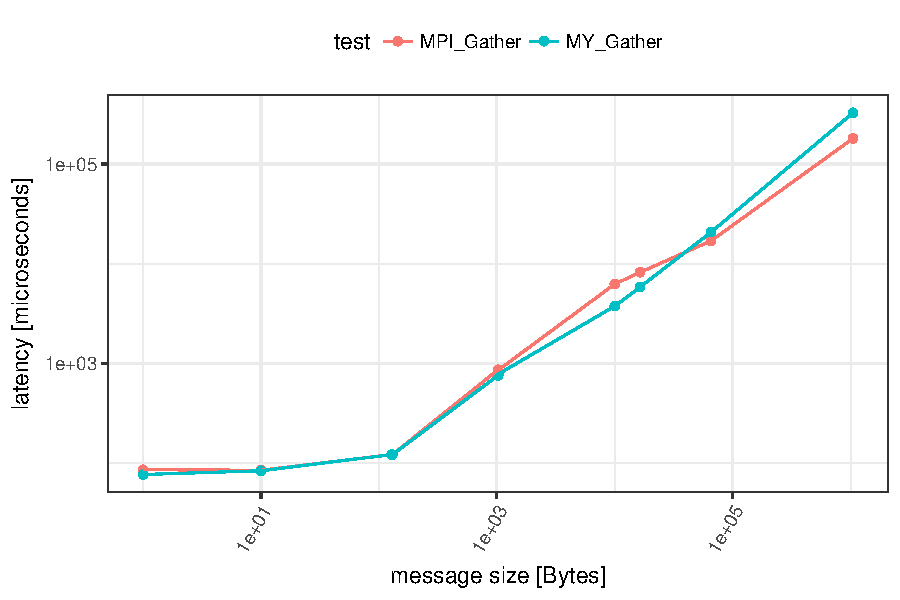
\includegraphics[width=\textwidth]{../benchmarks/openmpi/binom/gather_32/runtime.pdf}
        \caption{Binomial-Tree Implementation}
    \end{subfigure}
    \begin{subfigure}[b]{0.49\textwidth}
        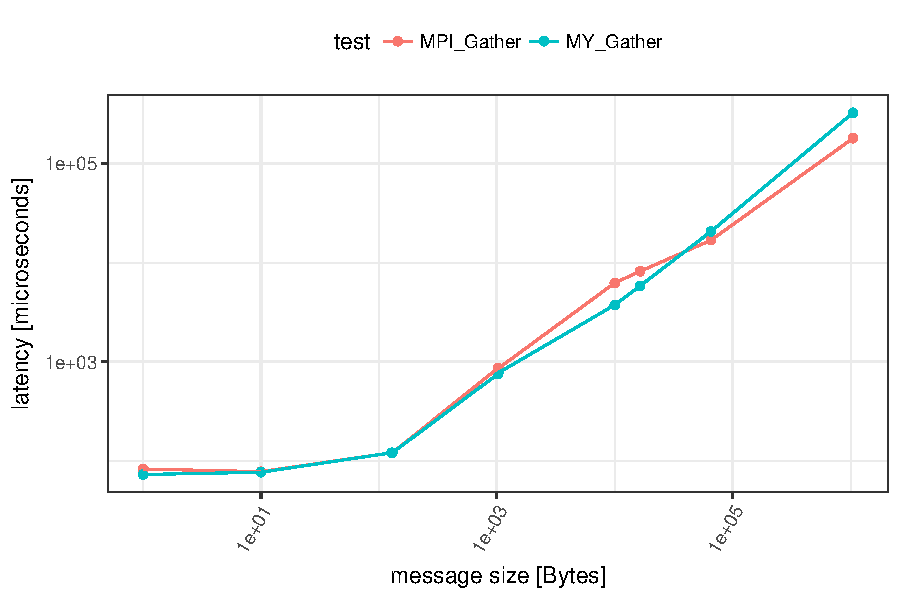
\includegraphics[width=\textwidth]{../benchmarks/openmpi/divide_conquer/gather32/runtime.pdf}
        \caption{Divide-And-Conquer Implementation}
    \end{subfigure}
    \caption{Comparison of Binomial Tree and Divide-And-Conquer Implementation}
    \label{fig:gather:binom_vs_dac}
\end{figure}

As seen, both algorithms perform similarly when the root node has rank 0. For the following discussions the binomial-tree implementation was chosen as the main strategy.

%-------
\subsection{Description / Strategy}

All processing nodes are organized in a binomial-tree with the root of the Gather algorithm as the root of the tree. Each leaf node sends its data to its parent node and all non-leaf nodes forward all received data and the data of the node itself to the parent. \\
Due to the use of a binomial tree, the calculation of the parent and child ranks can be done fast via bit-operations.\\

For cases where the root node has $rank \neq 0$, the algorithm uses virtual ranks:
$vrank = (rank - root - N ) \mod N$. In this case the data is received in virtual rank order at the root and has to be reordered to regain the real rank order.

\subsection{Round- and Bandwidth Optimality}

\subsubsection{Round Optimality}
Due to the tree structure nodes on the same level send data to their parent nodes in parallel, so each layer of the tree represents one communication round. Therefore the number of communications rounds is limited by $\mathcal{O}(log(p))$.

\subsubsection{Bandwidth Optimality}
Per round at most $2^{log(p)-1} \frac{m}{p}$ units of data are sent. % TODO

%-------
\subsection{Harmful Algorithmic Latency}
No Algorithmic Latency: Due to the calculation of child and parent nodes via bit operations, each processor can start to send/receive after $\mathcal{O}(1)$ steps.


%----------------------------------------------------------------------
\section{Algorithm \myscatter}

%-------
\subsection{Strategy Comparison}

\subsubsection{Binomial Tree}

\subsubsection{Divide-And-Conquer}

%-------
\subsection{Description / Strategy}

%-------
\subsection{Round- and Bandwidth Optimality}

%-------
\subsection{Harmful Algorithmic Latency}

%----------------------------------------------------------------------
\section{Experimental Results}

%-------
\subsection{Experiments and Discussion -- \mygather}

\begin{figure}[h]
    \centering
    
    \begin{subfigure}[b]{0.49\textwidth}
        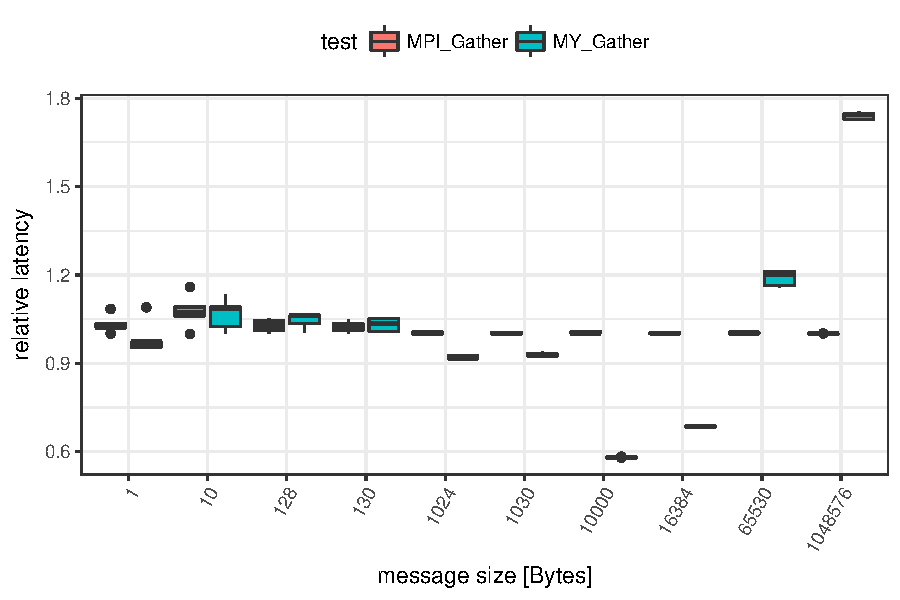
\includegraphics[width=\textwidth]{../benchmarks/openmpi/binom/gather_31/rel_runtime.pdf}
        \caption{Relative Runtime with $p=31 \times 16$}
        \label{fig:Gather:OpenMPI:Rel:31}
    \end{subfigure}
    \begin{subfigure}[b]{0.49\textwidth}
        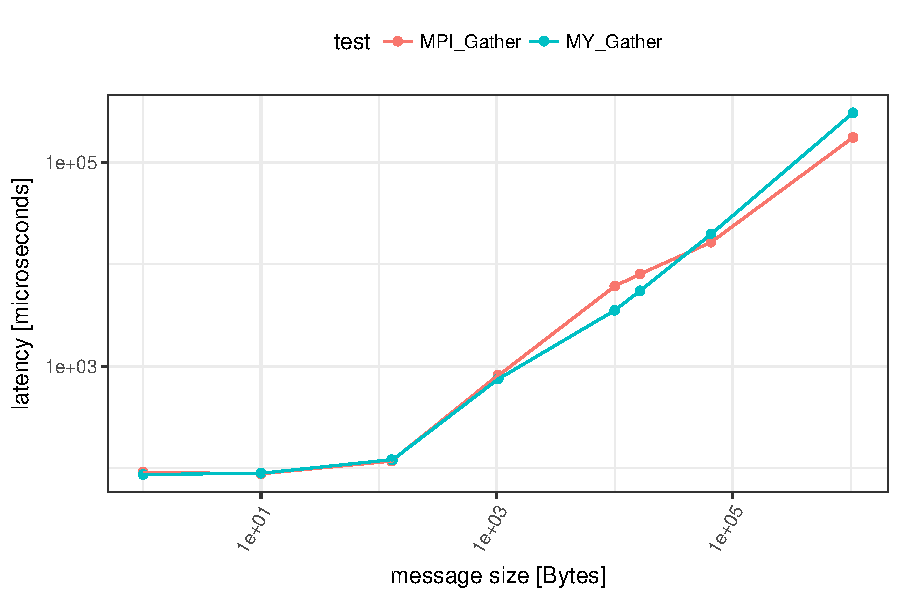
\includegraphics[width=\textwidth]{../benchmarks/openmpi/binom/gather_31/runtime.pdf}
        \caption{Absolute Runtime with $p=31 \times 16$}
        \label{fig:Gather:OpenMPI:Abs:31}
    \end{subfigure}
    
    \begin{subfigure}[b]{0.49\textwidth}
        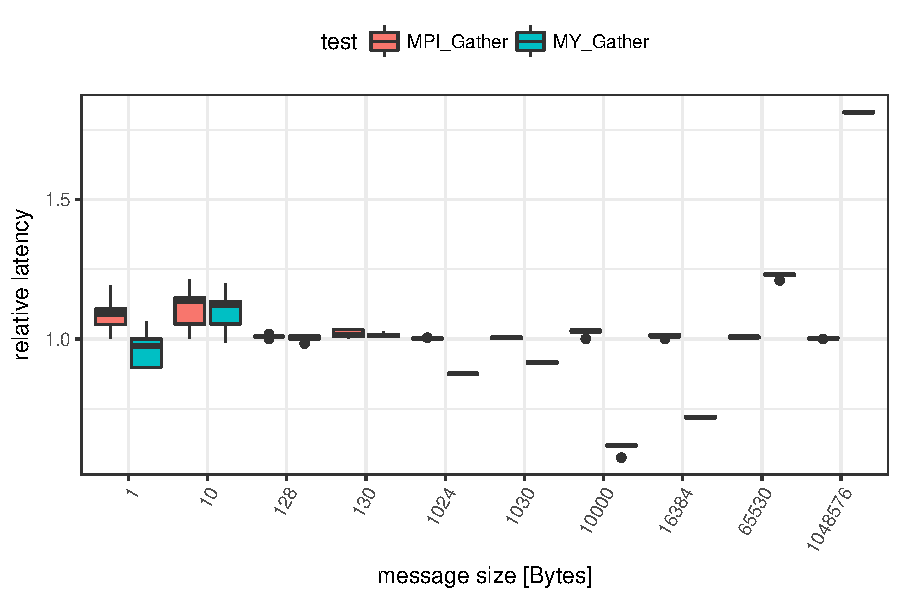
\includegraphics[width=\textwidth]{../benchmarks/openmpi/binom/gather_32/rel_runtime.pdf}
        \caption{Relative Runtime with $p=32 \times 16$}
        \label{fig:Gather:OpenMPI:Rel:32}
    \end{subfigure}
    \begin{subfigure}[b]{0.49\textwidth}
        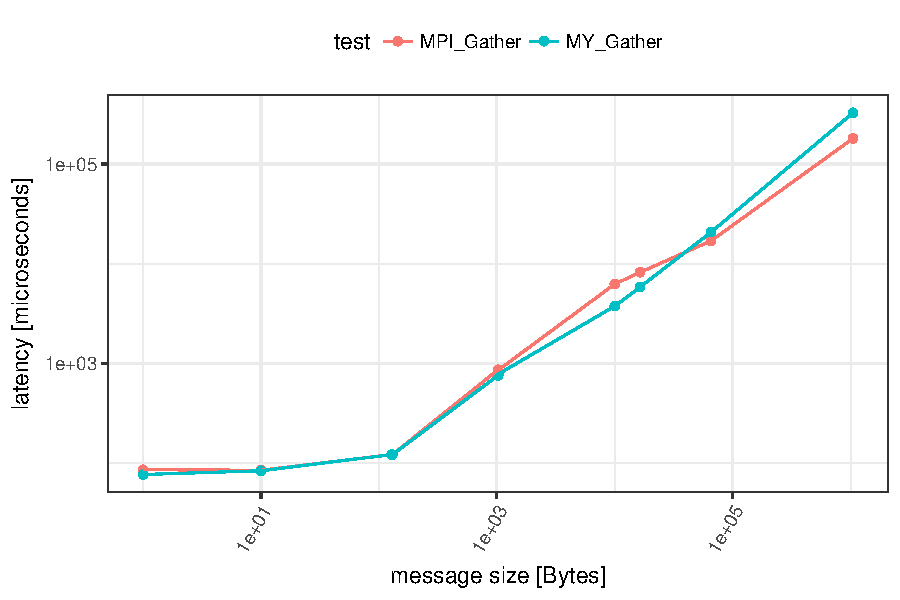
\includegraphics[width=\textwidth]{../benchmarks/openmpi/binom/gather_32/runtime.pdf}
        \caption{Absolute Runtime with $p=32 \times 16$}
        \label{fig:Gather:OpenMPI:Abs:32}
    \end{subfigure}
    
    \caption{\mygather compared to \mpigather of \texttt{Open MPI 1.10.3}}
\end{figure}

\begin{figure}[h]
    \centering
    
    \begin{subfigure}[b]{0.49\textwidth}
        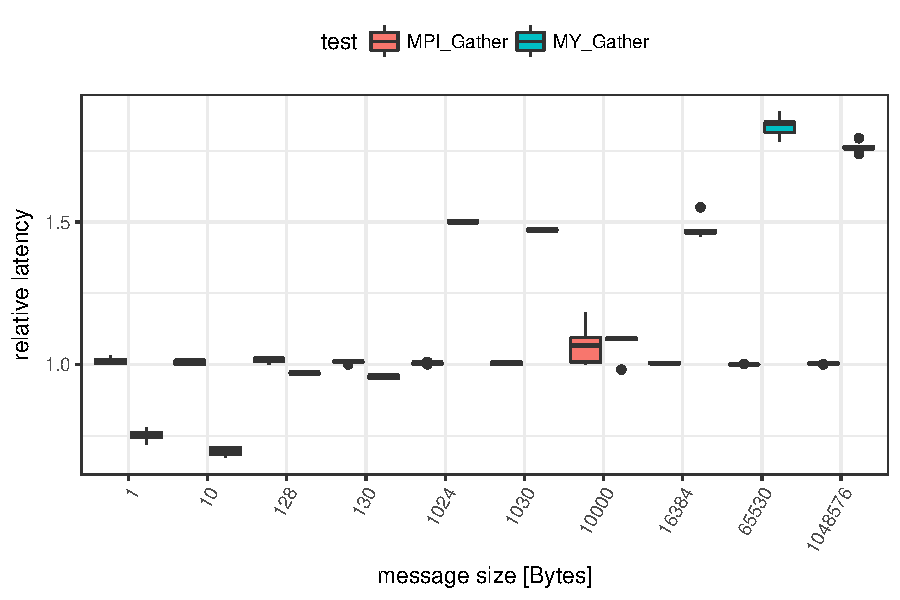
\includegraphics[width=\textwidth]{../benchmarks/mpich/binom/gather_31/rel_runtime.pdf}
        \caption{Relative Runtime with $p=31 \times 16$}
        \label{fig:Gather:MPICH:Rel:31}
    \end{subfigure}
    \begin{subfigure}[b]{0.49\textwidth}
        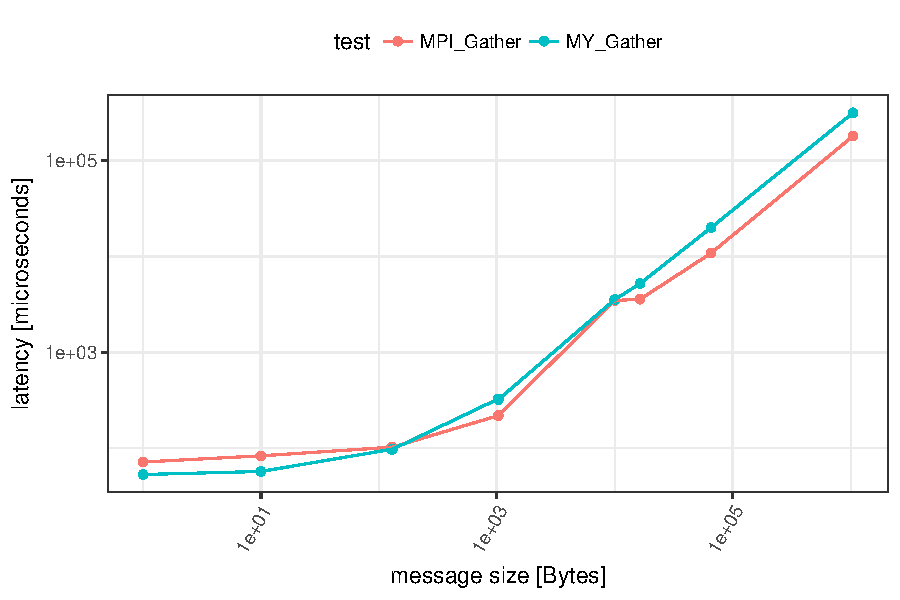
\includegraphics[width=\textwidth]{../benchmarks/mpich/binom/gather_31/runtime.pdf}
        \caption{Absolute Runtime with $p=31 \times 16$}
        \label{fig:Gather:MPICH:Abs:31}
    \end{subfigure}
    
    \begin{subfigure}[b]{0.49\textwidth}
        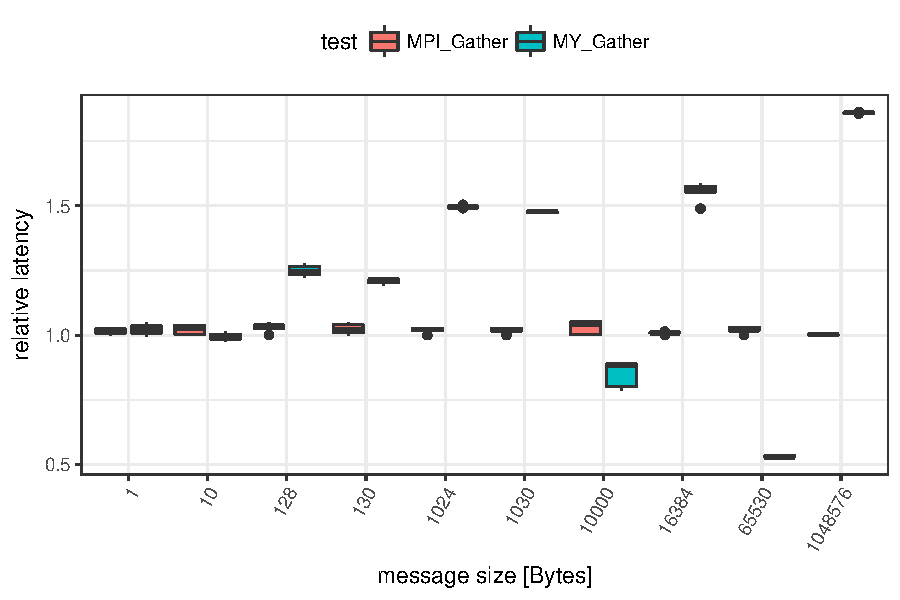
\includegraphics[width=\textwidth]{../benchmarks/mpich/binom/gather_32/rel_runtime.pdf}
        \caption{Relative Runtime with $p=32 \times 16$}
        \label{fig:Gather:MPICH:Rel:32}
    \end{subfigure}
    \begin{subfigure}[b]{0.49\textwidth}
        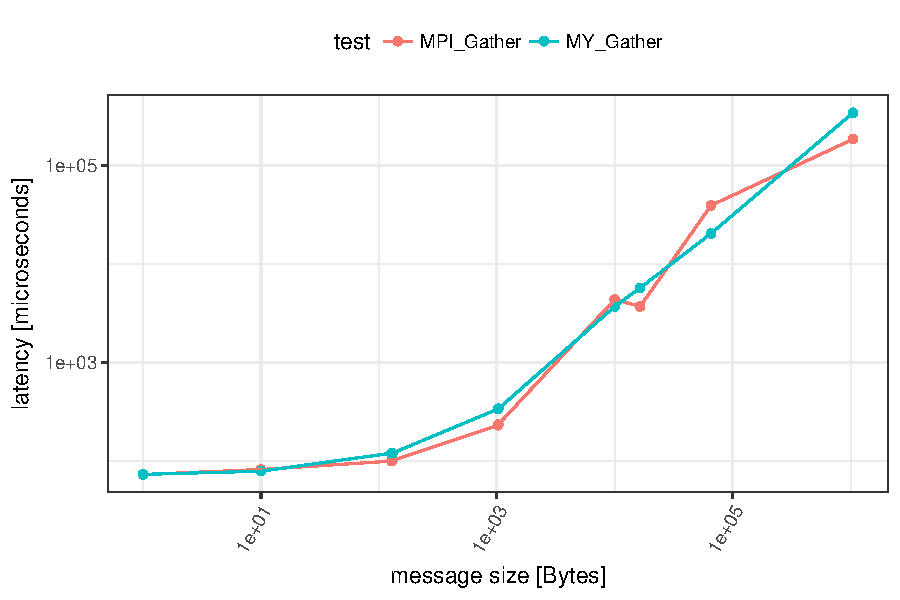
\includegraphics[width=\textwidth]{../benchmarks/mpich/binom/gather_32/runtime.pdf}
        \caption{Absolute Runtime with $p=32 \times 16$}
        \label{fig:Gather:MPICH:Abs:32}
    \end{subfigure}
    
    \caption{\mygather compared to \mpigather of \texttt{MVAPICH2 2.2}}
\end{figure}

%-------
\subsection{Experiments and Discussion -- \myscatter}

\begin{figure}[h]
    \centering
    
    \begin{subfigure}[b]{0.49\textwidth}
        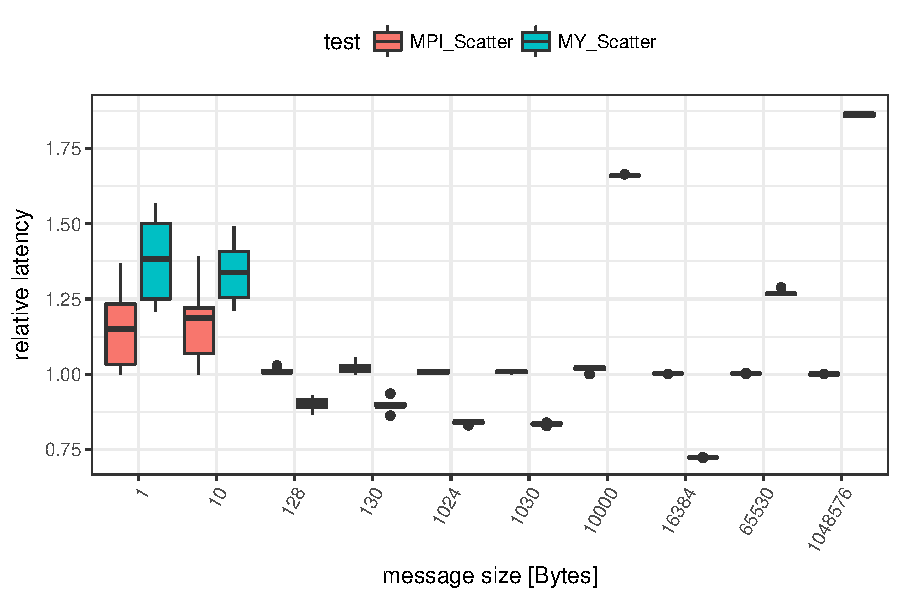
\includegraphics[width=\textwidth]{../benchmarks/openmpi/divide_conquer/scatter_31/rel_runtime.pdf}
        \caption{Relative Runtime with $p=31 \times 16$}
        \label{fig:Scatter:OpenMPI:Rel:31}
    \end{subfigure}
    \begin{subfigure}[b]{0.49\textwidth}
        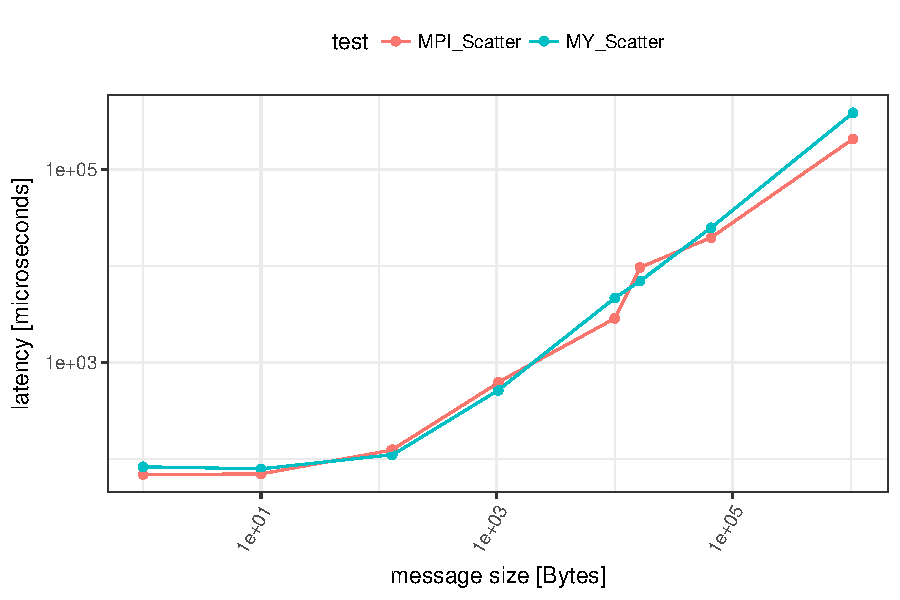
\includegraphics[width=\textwidth]{../benchmarks/openmpi/divide_conquer/scatter_31/runtime.pdf}
        \caption{Absolute Runtime with $p=31 \times 16$}
        \label{fig:Scatter:OpenMPI:Abs:31}
    \end{subfigure}
    
    \begin{subfigure}[b]{0.49\textwidth}
        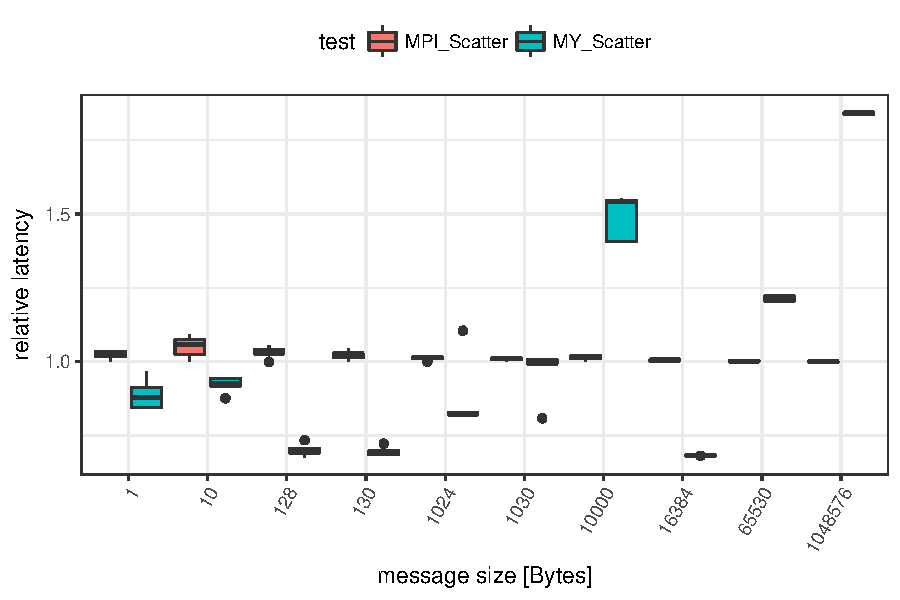
\includegraphics[width=\textwidth]{../benchmarks/openmpi/divide_conquer/scatter_32/rel_runtime.pdf}
        \caption{Relative Runtime with $p=32 \times 16$}
        \label{fig:Scatter:OpenMPI:Rel:32}
    \end{subfigure}
    \begin{subfigure}[b]{0.49\textwidth}
        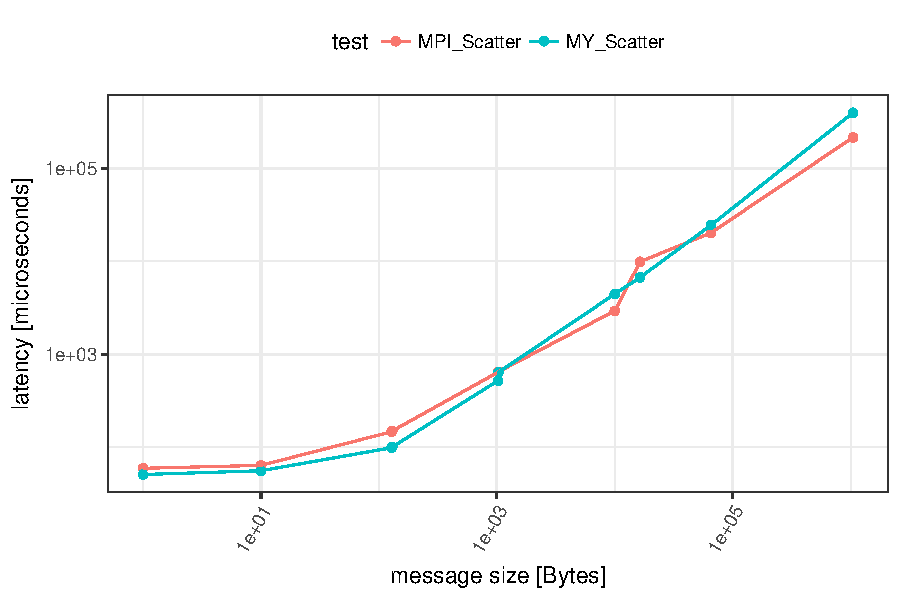
\includegraphics[width=\textwidth]{../benchmarks/openmpi/divide_conquer/scatter_32/runtime.pdf}
        \caption{Absolute Runtime with $p=32 \times 16$}
        \label{fig:Scatter:OpenMPI:Abs:32}
    \end{subfigure}
    
    \caption{\myscatter compared to \mpiscatter of \texttt{Open MPI 1.10.3}}
\end{figure}

\begin{figure}[h]
    \centering
    
    \begin{subfigure}[b]{0.49\textwidth}
        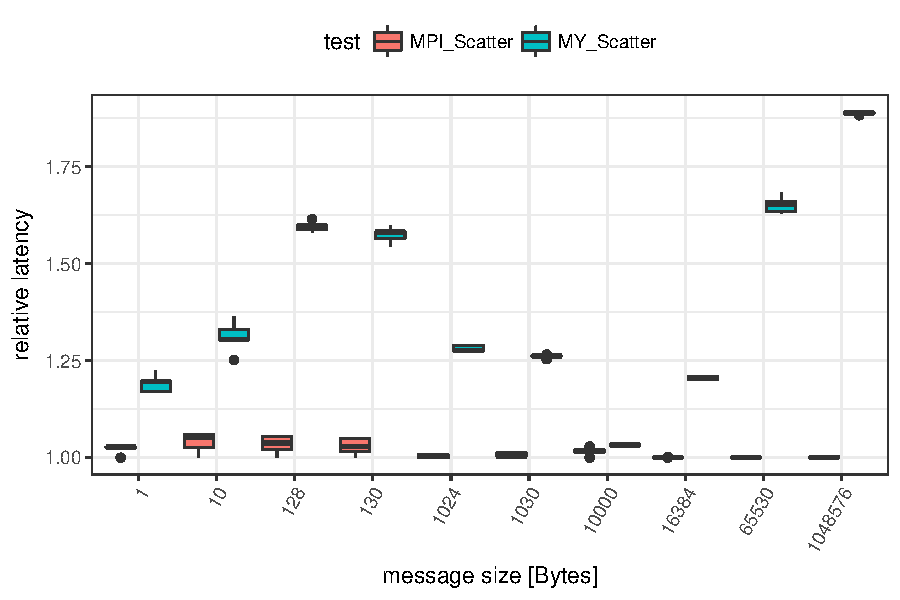
\includegraphics[width=\textwidth]{../benchmarks/mpich/divide_conquer/scatter_31/rel_runtime.pdf}
        \caption{Relative Runtime with $p=31 \times 16$}
        \label{fig:Scatter:MPICH:Rel:31}
    \end{subfigure}
    \begin{subfigure}[b]{0.49\textwidth}
        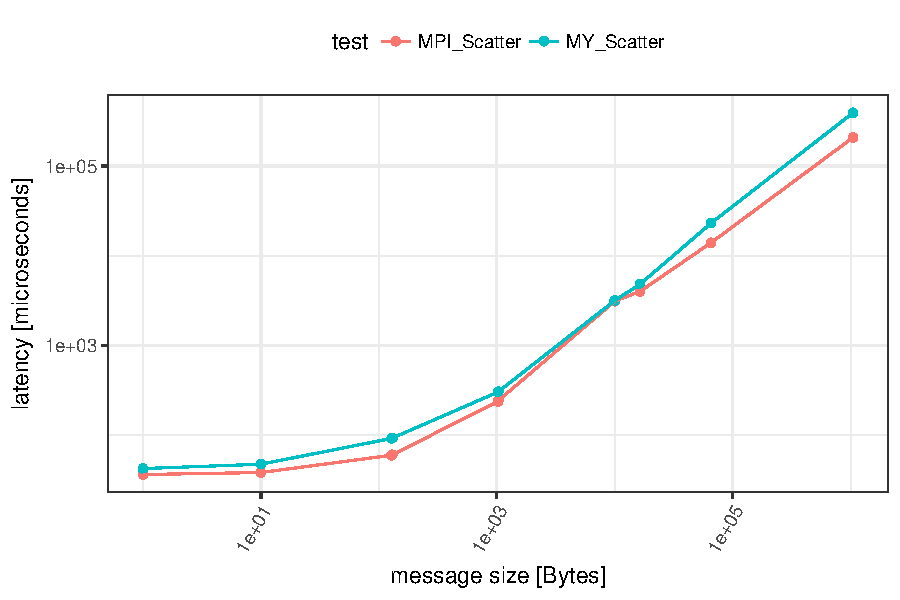
\includegraphics[width=\textwidth]{../benchmarks/mpich/divide_conquer/scatter_31/runtime.pdf}
        \caption{Absolute Runtime with $p=31 \times 16$}
        \label{fig:Scatter:MPICH:Abs:31}
    \end{subfigure}
    
    \begin{subfigure}[b]{0.49\textwidth}
        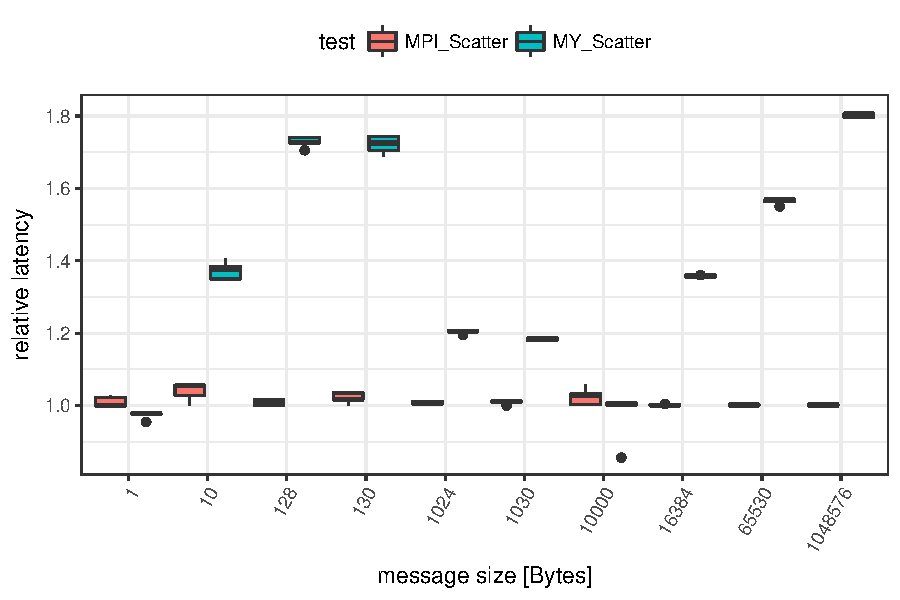
\includegraphics[width=\textwidth]{../benchmarks/mpich/divide_conquer/scatter_32/rel_runtime.pdf}
        \caption{Relative Runtime with $p=32 \times 16$}
        \label{fig:Scatter:MPICH:Rel:32}
    \end{subfigure}
    \begin{subfigure}[b]{0.49\textwidth}
        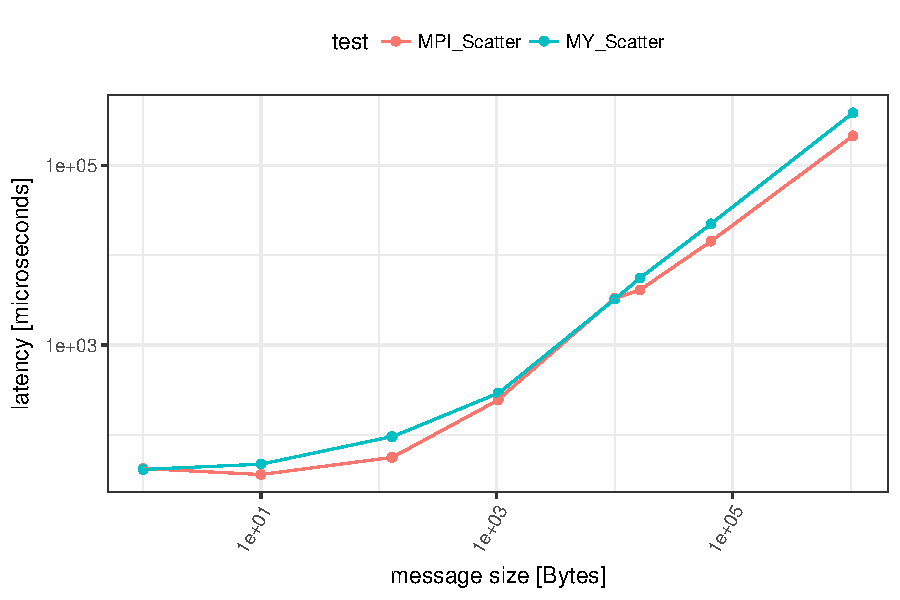
\includegraphics[width=\textwidth]{../benchmarks/mpich/divide_conquer/scatter_32/runtime.pdf}
        \caption{Absolute Runtime with $p=32 \times 16$}
        \label{fig:Scatter:MPICH:Abs:32}
    \end{subfigure}
    
    \caption{\myscatter compared to \mpiscatter of \texttt{MVAPICH2 2.2}}
\end{figure}